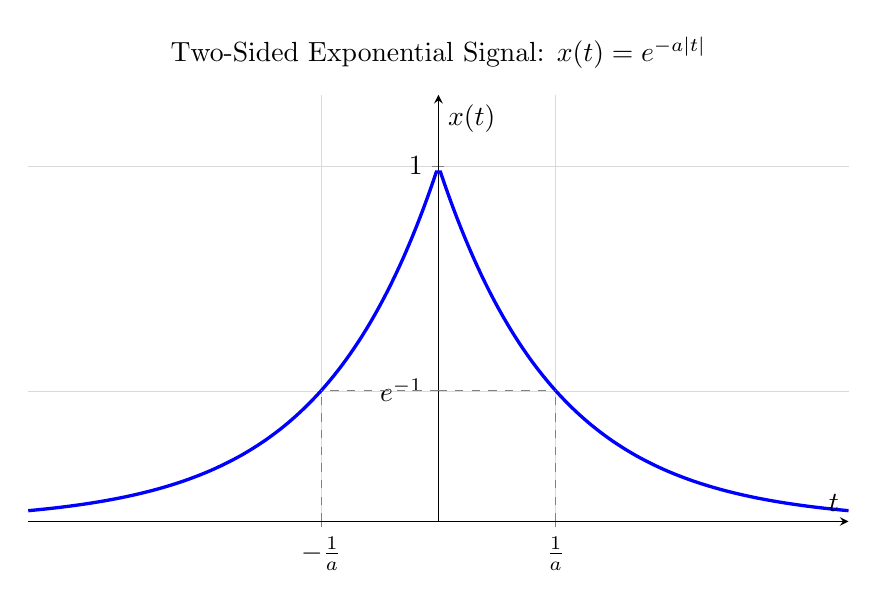
\begin{tikzpicture}
	\begin{axis}[
		width=12cm,
		height=7cm,
		title={Two-Sided Exponential Signal: $x(t) = e^{-a|t|}$},
		xlabel={$t$},
		ylabel={$x(t)$},
		axis lines=middle,
		xmin=-3.5, xmax=3.5,
		ymin=0, ymax=1.2,
		xtick={-1, 1},
		xticklabels={$-\frac{1}{a}$, $\frac{1}{a}$},
		ytick={0.3678, 1},
		yticklabels={$e^{-1}$, $1$},
		grid=major,
		grid style={line width=.1pt, draw=gray!30},
		]
		
		% Plot the function for a=1
		\addplot[blue, very thick, domain=-3.5:3.5, samples=200, no marks] {exp(-abs(x))};
		
		% Add guidelines
		\draw[dashed, gray] (axis cs:1,0) -- (axis cs:1, {exp(-1)});
		\draw[dashed, gray] (axis cs:-1,0) -- (axis cs:-1, {exp(-1)});
		\draw[dashed, gray] (axis cs:0,{exp(-1)}) -- (axis cs:1,{exp(-1)});
		\draw[dashed, gray] (axis cs:0,{exp(-1)}) -- (axis cs:-1,{exp(-1)});
		
	\end{axis}
\end{tikzpicture}